% Convert with command:
% convert -density 300 pic.pdf -quality 90 pic.png
\documentclass[crop,tikz,border=0pt]{standalone}
\usetikzlibrary{arrows.meta}
\begin{document}
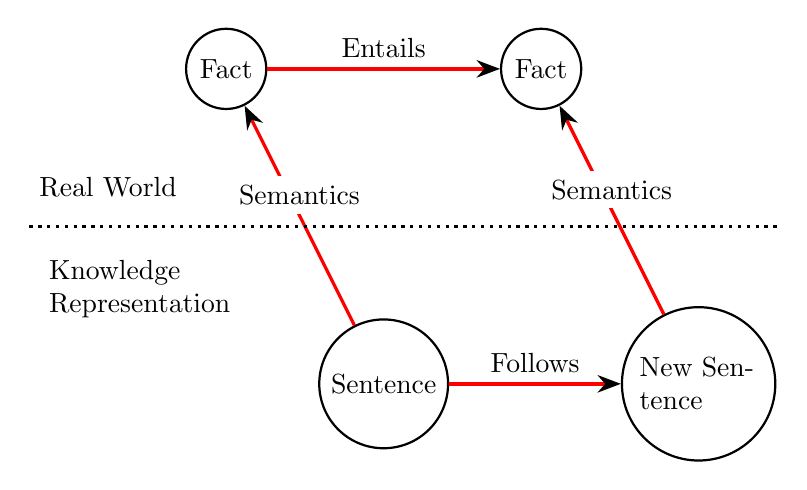
\begin{tikzpicture}

\begin{scope}[every node/.style={circle,thick,draw}]

    \node (A) at (0, 0) [shape=circle, fill=white] {Fact};
    \node (B) at (4, 0) [shape=circle, fill=white] {Fact};

    \node (C) at (2, -4) [shape=circle, fill=white] {Sentence};
    \node (D) at (6, -4) [shape=circle, fill=white, text width=15mm] {New Sentence};
    % \draw (0,0) rectangle (4,4) [fill=white] {};
    % \draw (5,0) rectangle (9,4) [fill=white] {};

    % \node (A) at (2,3.5)[shape=rectangle, fill=white] {State};
    % \node (B) at (2,1.5)[shape=rectangle, fill=white] {Knowledge Base};

    % \node (C) at (7,3.5)[shape=rectangle, fill=white] {Sensors};
    % \node (D) at (7,1.5)[shape=rectangle, fill=white] {Actuators};
\end{scope}


\begin{scope}[>={Stealth[black]},
              every node/.style={fill=white,rectangle,above},
              every edge/.style={draw=red,very thick}
]
    \path [->] (A) edge node {Entails} (B);
    \path [->] (C) edge node {Semantics} (A);
    \path [->] (D) edge node {Semantics} (B);
    \path [->] (C) edge node {Follows} (D);
\end{scope}

\path [-] (-2.5, -2) edge [very thick, dotted] node {} (7, -2);

\draw (-1.5,-1.5) node [text=black] {Real World};
\draw (-1,-2.8) node [text=black, text width=25mm] {Knowledge Representation};

\end{tikzpicture}
\end{document}
